\chapter{The Design of \emph{GrowFlesh}}
In this chapter I will explain the internals of \emph{GrowFlesh}. I will outline the data structure I used for the model, and some of the interesting algorithms I desinged to calculate inter- and intra- cellular forces. It is interesting to note that a number of datastructures and algorithms were scrapped in the beginning of the modeling process because of the complicated relationship between and vertices. The model I have implemented is a vertex dynamics model, and, as such, one would think that the main object of interest should be a vertex. Vertices require information about the cells which contain them in order to be moved. With this as a starting idea, I developed a sophisticated vertex class which contained cells as member variables. Apart from the software bloat coming from many vertices containing massive amounts of cell information, another issue was that cells are made of vertices, and, as such, cells ought to contain vertices as member variables! Unfortunately this bilateral inclusion is not supported by C++. In this chapter I will describe how this issue was circumvented through the use of tables which mimic the behavior of a relational database.

\section{[Highly Simplified] Pseudocode}
Here I will briefly outline how the code works. All of the functions are explained in some detail later in this chapter.
\begin{lstlisting}
mesh_variables $<$- read_configs()
mesh $<$- make_mesh()
random_alterations(mesh)
copy(mesh, rotate_mesh)
rotate(rotate_mesh)
print(simulation_info) # So the user can verify all parameters.
for i = 1:num_iters
   if(iter%print_freq == 0)
      print(OFF_file)
   temp_mesh = NagaiHondaForce(mesh) # if any displacement in temp_mesh,
                                     # the displacement is recalculated
   temp_rotate_mesh = NagaiHondaForce(rotate_mesh)
   mesh $<$- mesh + temp_mesh
   rotate_mesh $<$- rotate_mesh + temp_rotate_mesh
   performT1(mesh)
   performT2(mesh)
   performT1(rotate_mesh)
   performT2(temp_rotate_mesh)
rotate_back(rotate_mesh)
compare_mesh(mesh, rotate_mesh)
print(graphs and error analysis)
\end{lstlisting}

\section{Classes}
\emph{GrowFlesh} uses two classes to organize data. They are the cell and coordinate classes.
\subsection{The Cell Class}
The cell class contains a number of useful functions and data members to make the code easy to read and understand. All cell information could have been stored in arrays, but the OO structure makes the code more readable. All cells know their index, which vertices (coordinates) make them up, they are able to calulate their area and perimeter, can modify their constituent vertices, can tell you whether or not ther contain a vertex, and can print out a graphical, color coded representation of themselves to an OFF file.
\begin{lstlisting}
public:
 cell(int index, vector$<$int$>$ AssociatedVertices,\
       double target_area = t_area, double gamma = t_gamma)
 {	
   assert(index $>$= 0);
   m_AssociatedVertices = AssociatedVertices;
   m_index = index;
   m_target_area = target_area;
   m_target_perimeter = sqrt(pi * m_target_area);
   m_gamma = gamma; 
 }
	
 cell(){} // Default constructor
	
 vector$<$int$>$ GetVertices(){return m_AssociatedVertices;};
 int GetIndex(){return m_index;};
 void SetIndex(int index){m_index = index;};
 void SetTargetArea(double area){m_target_area = area;};
 double GetTargetArea(){return m_target_area;};
 double GetTargetPerimeter(){return m_target_perimeter;};
 double ComputeArea(double * X, double * Y);
 double ComputePerimeter(double * X, double * Y);
 void PrintCell(ofstream &OffFile);
 int ContainsVertex(int index);
 void SetGamma(double gamma){m_gamma = gamma;};
 double GetGamma(){return m_gamma;};
 void InsertVert(int v1, int v2);
 void EraseVert(int index)
 {
   vector$<$int$>$::iterator it = find(m_AssociatedVertices, index); 
   m_AssociatedVertices.erase(it);
 };
 void ReplaceVert(int before, int after)
 {
   vector$<$int$>$::iterator it = find(m_AssociatedVertices, before); 
   *it = after;
 };
 void SetVertices(vector$<$int$>$ vertices)
 {
   m_AssociatedVertices = vertices;
 };
 int GetNumSides(){return m_AssociatedVertices.size();};
private:
 vector$<$int$>$ m_AssociatedVertices; // Stored counterclockwise
 int m_index;	
 double m_target_area;
 double m_target_perimeter;
 double m_gamma;
};

\end{lstlisting}

\subsection{The Coordinate Class}
The coordinate class stores the index of a coordinate, and whether or not the vertex will move during the integration. \emph{GrowFlesh} will run with two types of meshes: meshes with border, and meshes without. A mesh with border is a mesh with fixed border elements. A mesh without border is a mesh which was generated with periodic boundary conditions and which maintains the periodicity throughout the calculations done by the program. Border vertices will not move, whereas interior vertices will be able to move; the coordinate class allows us to secify whether or not a vertex is interior or exterior. Another benefit of this class is that is allows use to easily extend the code to include forces acting on individual vertices, and to specify other types of vertices besides interior and exterior. This code was developed with eyes to the future. Another interesting idea to explore in computational biology is active cell migration, ad the cell class allows us to specify which vertices want to move actively.
\begin{lstlisting}
class coordinate
{
public:
  coordinate(int idx, bool t) : index(idx), IsInner(t){};
  coordinate(){index = -1; IsInner = 0;};
  int index;
  bool IsInner;
  inline bool operator==(const coordinate& rhs)
  {return index == rhs.index;};
};
\end{lstlisting}

\section{Initial Mesh Design}
The hex\_mesh() function generates an $n$x$n$ mesh of cells, where the dimension represents the number of cells touching the boundary. 

\begin{figure}
\centering
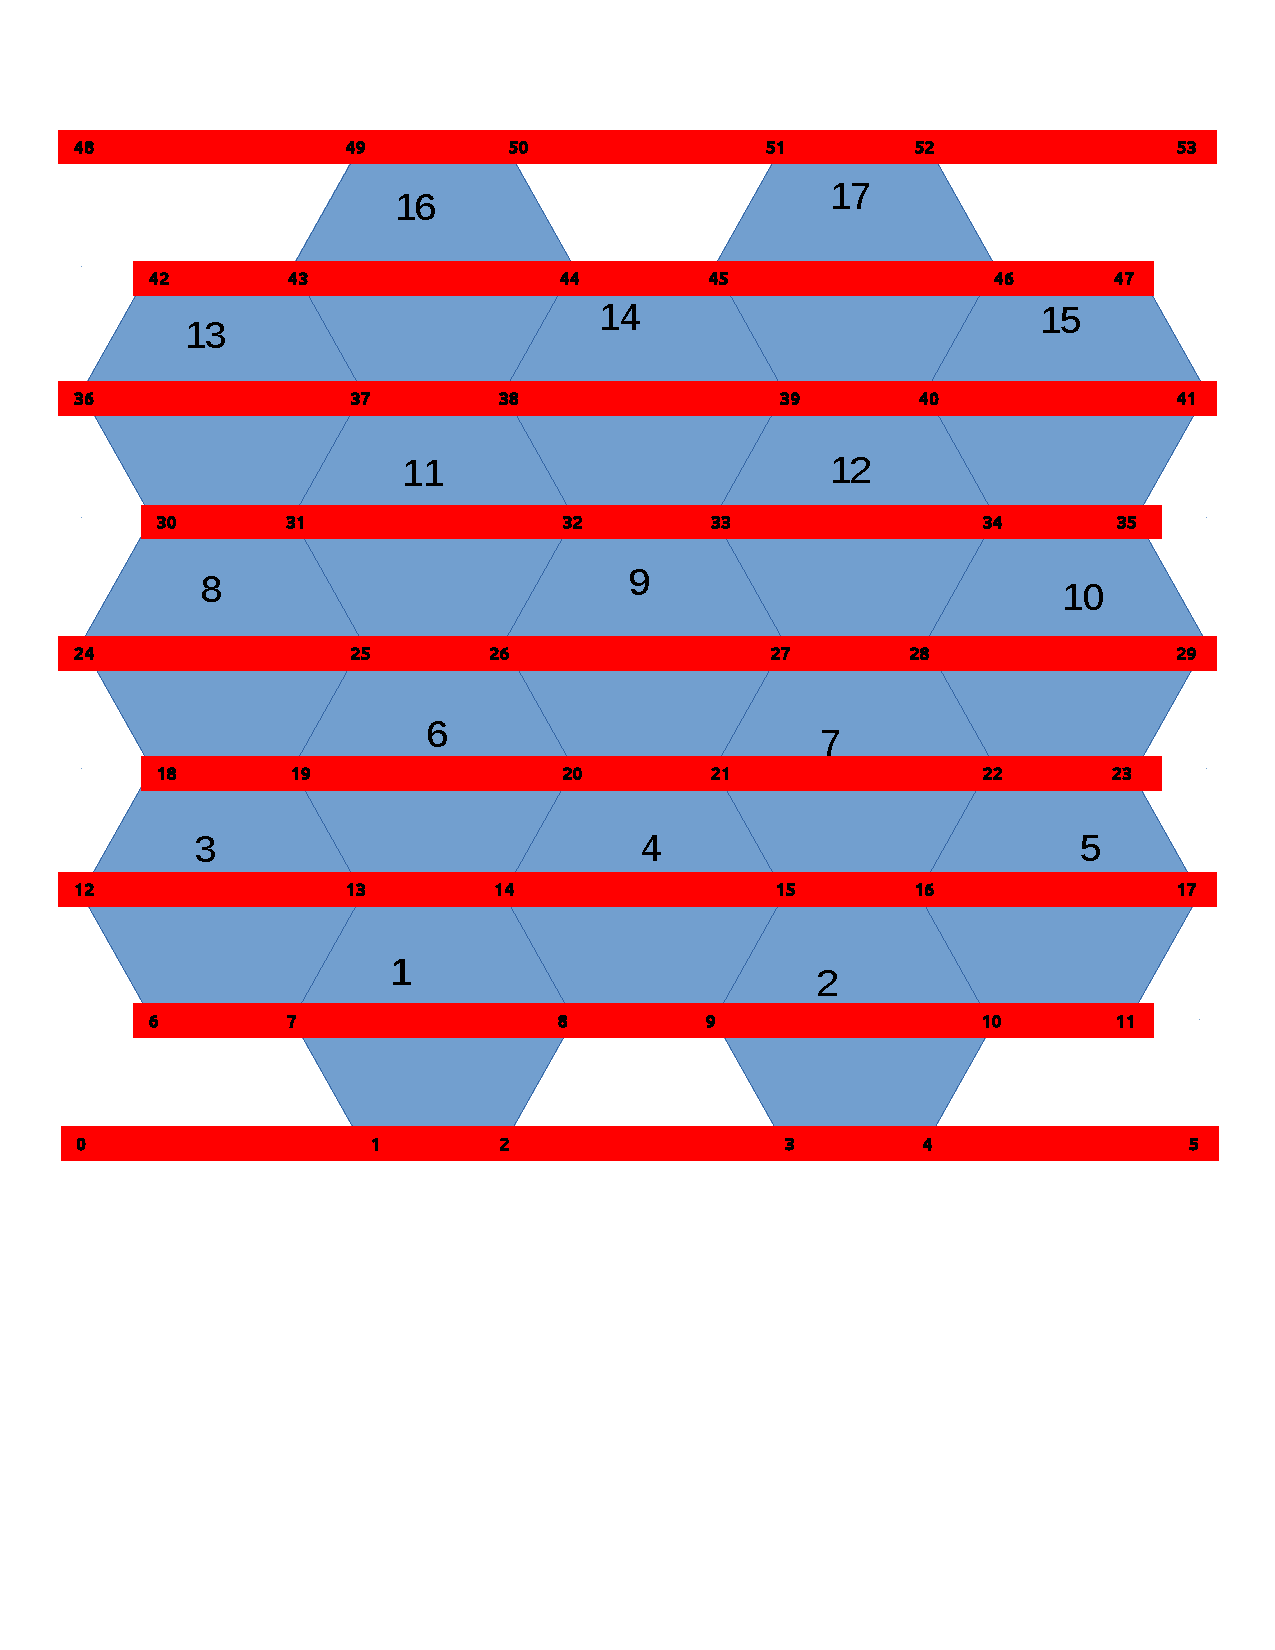
\includegraphics[height=0.7\textheight]{../diagrams/vert_mesh.pdf}
\caption[A 5x5 Hexagonal Mesh.]{A 5x5 hexagonal mesh. The cell indices are written in the cells and the vertex indices are written on the red bars.}
\label{fig:mesh}
\end{figure}

\section{A Relational Database}
A popular way to store data since the 1970's is to store data in group of tables which are connected via \emph{keys}. This type of database is popular for reasons which will become apparent by means of a simple example. 

Consider a business which sells a number of products, and wants to keep track of their customers, the customer's orders, the customer's addresses, and information about the products ordered. A wasteful way to store this data is to store a large table with a column for customer. Next to every customer's name is the customer's address. Next to the customers address is the customer's order number. Next to the customer's order number is an item in that order. And, next to each item ordered is the item information. This method of storing data is terribly redundant, for each customer you would need $\sum\limits_{c}\sum\limits_{o_c}|o_c|$ rows in the table, and many rows would have the customer's information repeated. Similarly, item information would be repeated in every row that features this item. 

A better idea is to break this data up into several tables which together define a \emph{schema}. In this example, the following tables define a good schema:
\begin{enumerate}
\item Customer information. columns: name, address, order number
\item Order numbers: columns: order number, item
\item Items: columns: item, item description
\end{enumerate}

We are now guaranteed that the customer information is not duplicated for every item in an order, and that item information is not duplicated every time an item is in an order.

\begin{figure}[h]
\centering
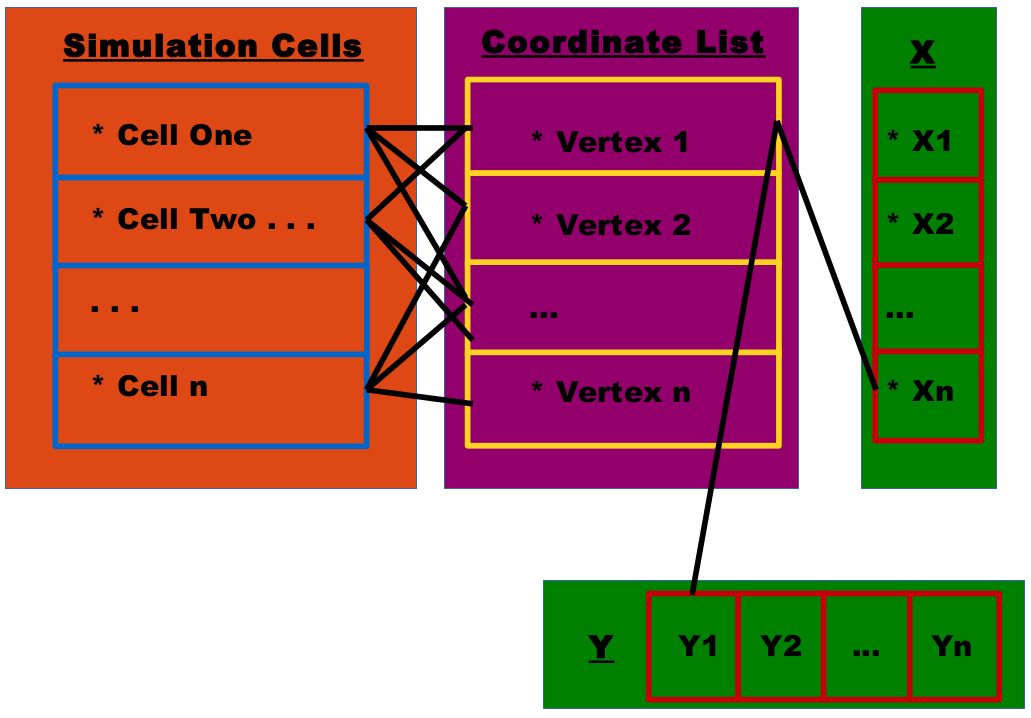
\includegraphics[width=0.5\textwidth]{../diagrams/ds.png}
\caption{The Relational Database}
\end{figure}

My data structure is inspired by the relational database model. I have six tables, including the simulationCells, coordinateList, X, Y, tempX and tempY tables. The cell and coordinate tables are implemented as 1d vectors of cell and coordinate indices, whereas the position tables are implemented as 1d arrays for ease of passing these structures to CUDA C functions (will talk more about CUDA C later). The cells can extract coordinate information from the coordinateList table via the \emph{index} key, and the coordinateList can access the position information from the X and Y arrays via their own \emph{index}. The temporary X and Y arrays store temporary position information about the vertices before the mesh positions are updated. This choice saves memory because the cells, coordinates, and coordinate locations are stored independently of each other, and there is no data redundancy. 

\section{Moving the Vertices}
\emph{GrowFlesh} loops over the vertices, computes the force applied to each vertex and then computes a displacement due to the force using the Euler Method. In their original paper, H. Honda and T. Nagai described the use of a Modified Runge Kutta Method to move the vertices, but this method would result in extra unnecessary computations at each time step. The \emph{Error Tolerance} section of this chapter describes how the Euler Method is numerically stable enough for this application. The same decision to use then Euler Method was made by the research group at Oxford that developed CHASTE, the \emph{other} leading software for implementing the Nagai-Honda Model. 

A displacement is calculated and stored in the temporary X and Y arrays. No vertex is permitted to move more than one half of the minimum delta separating vertices (the $\delta$ under which a T1 swap will occur) during an integration. By imposing this restiction we are ensuring that we will not miss the event of two vertices coming critcally close and a T1 swap occurring. Also, this prevents vertices from passing each other and invalidating the mesh. To ensure that no vertex moves too much, we store verify each displacement as we put it in the temporary X and Y arrays. If a displacement is too large, then the entire array of temporary displacements is erased, the time step is halved, and we begin the integration again. We could label the integrator as `fault tolerant'.

\begin{wrapfigure}{L}{0.4\textwidth}
\begin{center}
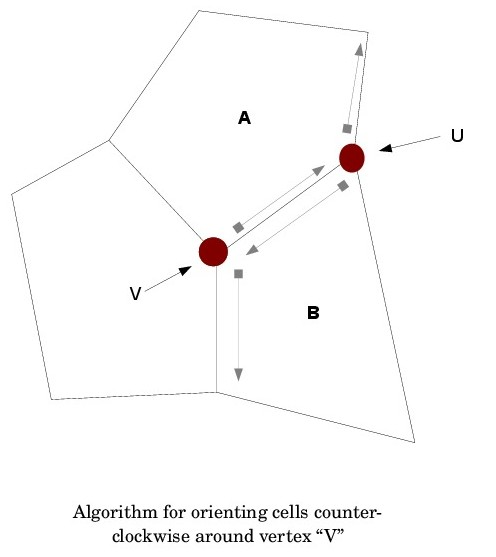
\includegraphics[width=0.38\textwidth]{../diagrams/counterclockwise.jpg}
\end{center}
\caption{Getting Cells in Order}
\label{fig:ctrclockwise}
\end{wrapfigure}

Another important aspect of the numerical integration is that cell and vertex information must be processed in counterclockwise order. In Figure~\ref{fig:ctrclockwise} I illustrate how a vertex can find the cells surrounding it in this order. When we are integrating a vertex $i$, the vertex first searches in the cell vector for a cell which contains it, and then the vertex finds the next vertex in that cell. Then, we have an edge. Some other cell contains that edge if it contains both of the vertices. That cell must be clockwise from the first. The cells are stored in the reverse order of which they are uncovered by this algorithm before the integration starts. This is a very expensive step ($O(n^3)$) in the computation, and ought to be optimized.


\section{Embarassing Parallelism and CUDA}
The numerical integrations and the vertex location updates exhibit what Cleve Moler describes as ``embarassing parallelism''. Computing the displacement of vertex \emph{a} does not depend upon the computation of the displacement of vertex \emph{b} during a given time step. Similarly, the vertex locations can all be updated in parallel since the update is simply a vector sum operation of the X and Y arrays with the temporary X and Y arrays, respectively. 

A popular hardware choice for parallel programming in last decade has been the NVIDIA GPU. CUDA is the NVIDIA extension of the C programming language which can run certain parts of C code on the GPU, while still running the serial and i/o operation on the CPU. I wrote some parts of the code in this language, and these parts were very simple to implement. The GPU is a collection of small processors, and the vertices are small, simple objects, so I mapped each vertex in the mesh to one of the hundreds of small processors to get some computational speedup.

Specifically, CUDA was employed to update vertex locations, since the sum of 1d arrays is well suited to a GPU. I also parallelized the rotation of the mesh and the reduction step which found the maximum error between the mesh and the rotated mesh. An interesting possibility is that of parallelizing the force computations. I was unable to do this with the code as it is because the cell data uses C++ vectors, while cuda only likes to take large C arrays as input. There is an interesting library called \emph{thrust} which can strips the vectors down to arrays and does all of the memory allocations for you, but the issue then becomes one of compiling the cells into one big vector with clever structure. This is left as a future project. 

CUDA was used to multiply each vertex in the mesh by the rotation matrix:
\[ \left( \begin{array}{cc}
\cos\theta & -\sin\theta \\
\sin\theta & \cos\theta 
\end{array} \right)\] 

\section{Computing Topological changes.}
\subsection{The T1 Swap}
The PerformT1s() function loops over all of the cells in the mesh, and checks the edge lengths in that cell. If an edge is critically small, then the other three cells involved in the junction are found. One of the two clashing vertices is deleted from the main cell, and the other clashing vertex is deleted from the neighboring cell. The midpoint of the critical edge is calculated, and then a perpendicular line is drawn through it. The vertices are then moved a distance $\delta/2$ into the interior of the cells ($\delta$ is the minimum vertex separation, and the vertices now have this minimal spacing). Then, these two vertices are inserted into the cells which previously hadn't been neighbors, making then adjacent after the swap. Figure ~\ref{fig:t1} offers a visual aid to understanding the swap. 

There are 8 cases to consider when inserting moving the vertices the distance $\delta/2$. I and Ip1 are the critically close vertices, where Ip1 comes before I in clockwise order in a cell. $mp$ is the midpoint of $\bar{(I, Ip1)}$. $dx$ and $dy$ are the displacements which will give a minimal separation after the swap. 
\begin{enumerate}
\item %1
\textbf{Given:}\\
I.x $<$ Ip1.x AND I.y == Ip1.y
\textbf{Then:}\\
I $\mapsto$ mp + (0, -dy) AND Ip1 $\mapsto$ mp + (0, dy)
\item %2
\textbf{Given:}\\
I.x $>$ Ip1.x AND I.y == Ip1.y
\textbf{Then:}\\
I $\mapsto$ mp + (0, dy) AND Ip1 $\mapsto$ mp + (0, -dy)
%%%%%%%%%%%%%%%%%%%%%%%%%%%%%%%%%%%%%%%%%%%%%%%%%%%%%%%%%%%
\item %3
\textbf{Given:}\\
I.x $<$ Ip1.x AND I.y $<$ Ip1.y
\textbf{Then:}\\
I $\mapsto$ mp + (dx, -dy) AND Ip1 $\mapsto$ mp + (-dx, dy)
\item %4
\textbf{Given:}\\
I.x $>$ Ip1.x AND I.y $>$ Ip1.y
\textbf{Then:}\\
I $\mapsto$ mp + (-dx, dy) AND Ip1 $\mapsto$ mp + (dx, -dy)
%%%%%%%%%%%%%%%%%%%%%%%%%%%%%%%%%%%%%%%%%%%%%%%%%%%%%%%%%%%
\item %5
\textbf{Given:}\\
I.x $<$ Ip1.x AND I.y $>$ Ip1.y
\textbf{Then:}\\
I $\mapsto$ mp + (-dx, -dy) AND Ip1 $\mapsto$ mp + (dx, dy)
\item %6
\textbf{Given:}\\
I.x $>$ Ip1.x AND I.y $<$ Ip1.y
\textbf{Then:}\\
I $\mapsto$ mp + (dx, dy) AND Ip1 $\mapsto$ mp + (-dx, -dy)
%%%%%%%%%%%%%%%%%%%%%%%%%%%%%%%%%%%%%%%%%%%%%%%%%%%%%%%%%%%
\item %7
\textbf{Given:}\\
I.x == Ip1.x AND I.y $>$ Ip1.y
\textbf{Then:}\\
I $\mapsto$ mp + (dx, -dy) AND Ip1 $\mapsto$ mp + (-dx, dy)
\item %8
\textbf{Given:}\\
I.x == Ip1.x AND I.y $<$ Ip1.y
\textbf{Then:}\\
I $\mapsto$ mp + (dx, -dy) AND Ip1 $\mapsto$ mp + (-dx, dy)
\end{enumerate}

\subsection{The implementation of the T2 swap.}
The PerformT2s() function looks at every cell in the mesh and checks its area. If the area is critically small, then the cell is deleted from the mesh. The centroid of the triangle is calculated, and this become the collapsed triangle. Then, one of the three vertices has its position updated to the centroid coordinate and any cell which contained on of the other two coordinates is assigned the centroid coordinate index as a replacement.

\section{Error Tolerance of the Algorithm}
\emph{GrowFlesh} has been empirically shown to be numerically stable; the code outputs an error measurement at the end of a simulation to give the user a sense of the stability. There was no clear way to provide an analytical proof of stability but at least we will always have an error measure to strengthen our confidence in the code. \emph{GrowFlesh} runs two simultions at the same time, one on the mesh made by hex\_mesh(), and another on the same mesh which has been rotated 45 degrees. Then, at the end of a simulation, the rotated mesh is rotated back and corresponding vertices are compared by index using the Euclidean norm. In practice we see near machine epsilon error for every simulation.

\begin{figure}[hr]
\centering
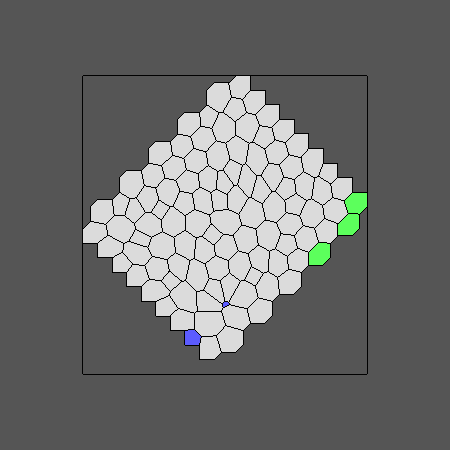
\includegraphics[width=0.5\textwidth]{../Images/rotate.png}
\caption{A Rotated Mesh for Error Analysis.}
\end{figure}